\documentclass{article}

\usepackage[utf8]{inputenc}

\usepackage{tikz}
\usetikzlibrary{petri}

\pagestyle{empty}

\begin{document}

\section*{Scenario 01}

A concrete Petri net is given, such as:
\begin{center}
  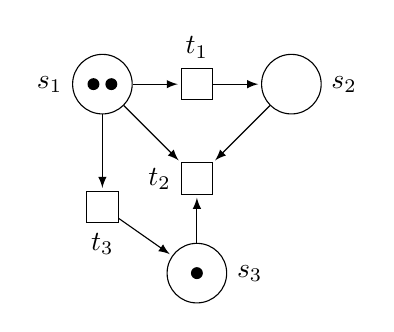
\begin{tikzpicture}[x=1.2cm,y=-1.2cm,baseline=(t1),>=latex]
    \node[place,tokens=2,label=left:$s_1$]  (s1) at (-1.0,0) {} ;
    \node[place,label=right:$s_2$] (s2) at ( 1.0,0) {} ;
    \node[place,tokens=1,label=right:$s_3$]          (s3) at (0,2) {} ;
    \node[transition,label=above:$t_1$] (t1) at (0,0) {}
    edge[pre]  (s1)
    edge[post] (s2) ;
    \node[transition,label=left:$t_2$] (t2) at (0,1) {}
    edge[pre] (s1)
    edge[pre] (s2)
    edge[pre] (s3);
    \node[transition,label=below:$t_3$] (t3) at (-1,1.3) {}
    edge[post] (s3)
    edge[pre] (s1) ;
  \end{tikzpicture}
\end{center}
and we want to use Alloy to report:
\begin{itemize}
\item
  Which transitions are activated?
\item
  Are there pairs of transitions in conflict? Which?
\item
  Are there pairs of transitions that are concurrently activated?
\item
  What is the maximum number of transitions concurrently activated?
\end{itemize}

\pagebreak

\section*{Scenario 02}

A Petri net structure, but without initial marking, is given, such as:
\begin{center}
  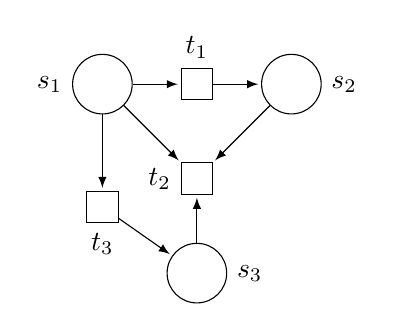
\begin{tikzpicture}[x=1.2cm,y=-1.2cm,baseline=(t1),>=latex]
    \node[place,label=left:$s_1$]  (s1) at (-1.0,0) {} ;
    \node[place,label=right:$s_2$] (s2) at ( 1.0,0) {} ;
    \node[place,label=right:$s_3$]          (s3) at (0,2) {} ;
    \node[transition,label=above:$t_1$] (t1) at (0,0) {}
    edge[pre]  (s1)
    edge[post] (s2) ;
    \node[transition,label=left:$t_2$] (t2) at (0,1) {}
    edge[pre] (s1)
    edge[pre] (s2)
    edge[pre] (s3);
    \node[transition,label=below:$t_3$] (t3) at (-1,1.3) {}
    edge[post] (s3)
    edge[pre] (s1) ;
  \end{tikzpicture}
\end{center}
and we want to use Alloy to find possible markings with certain properties.
Properties we might want to be able to impose (combinations of some of the following):
\begin{itemize}
\item
  Altogether at most, or exactly, $n$ tokens should be added.
\item
  In each place, at most $m$ tokens should be added.
\item
  A certain number $k$ of transitions are activated.
\item
  A specific transition $t$ is, or is not, activated.
\item
  There is no conflict.
\item
  There is a conflict between specific transitions $t$ and $t'$.
\item
  There are no concurrently activated transitions.
\item
  \dots
\end{itemize}

\pagebreak

\section*{Scenario 03}

A Petri net with an initial marking is given, such as:
\begin{center}
  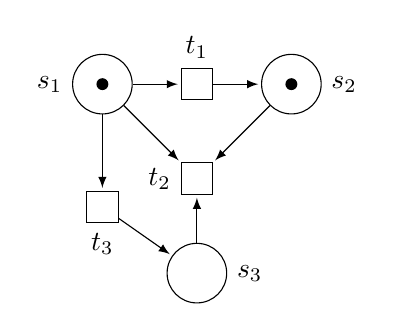
\begin{tikzpicture}[x=1.2cm,y=-1.2cm,baseline=(t1),>=latex]
    \node[place,tokens=1,label=left:$s_1$]  (s1) at (-1.0,0) {} ;
    \node[place,tokens=1,label=right:$s_2$] (s2) at ( 1.0,0) {} ;
    \node[place,label=right:$s_3$]          (s3) at (0,2) {} ;
    \node[transition,label=above:$t_1$] (t1) at (0,0) {}
    edge[pre]  (s1)
    edge[post] (s2) ;
    \node[transition,label=left:$t_2$] (t2) at (0,1) {}
    edge[pre] (s1)
    edge[pre] (s2)
    edge[pre] (s3);
    \node[transition,label=below:$t_3$] (t3) at (-1,1.3) {}
    edge[post] (s3)
    edge[pre] (s1) ;
  \end{tikzpicture}
\end{center}
and we want to use Alloy to solve tasks like the following:
\begin{itemize}
\item
  Add exactly one token somewhere so that two transitions are concurrently activated.
\item
  Remove a token so that there are no activated transitions.
% \item
%   Remove a token so that two previously concurrently activated transitions get into conflict.
\item
  \dots
\end{itemize}

\pagebreak

\section*{Scenario 04 (more advanced)}

A concrete Petri net is given, such as:
\begin{center}
  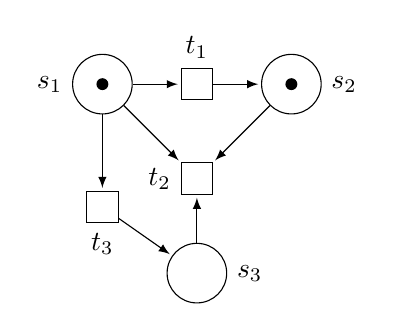
\begin{tikzpicture}[x=1.2cm,y=-1.2cm,baseline=(t1),>=latex]
    \node[place,tokens=1,label=left:$s_1$]  (s1) at (-1.0,0) {} ;
    \node[place,tokens=1,label=right:$s_2$] (s2) at ( 1.0,0) {} ;
    \node[place,label=right:$s_3$]          (s3) at (0,2) {} ;
    \node[transition,label=above:$t_1$] (t1) at (0,0) {}
    edge[pre]  (s1)
    edge[post] (s2) ;
    \node[transition,label=left:$t_2$] (t2) at (0,1) {}
    edge[pre] (s1)
    edge[pre] (s2)
    edge[pre] (s3);
    \node[transition,label=below:$t_3$] (t3) at (-1,1.3) {}
    edge[post] (s3)
    edge[pre] (s1) ;
  \end{tikzpicture}
\end{center}
and we want to use Alloy to solve tasks like the following:
\begin{itemize}
\item
  Change one incoming or outgoing weight of a transition (or add or remove an arrow) so that two transitions are concurrently activated.
\item
  Or: \dots\ so that there are no activated transitions.
% \item
%   Or: \dots\ so that two previously concurrently activated transitions get into conflict.
\item
  \dots
\end{itemize}

\pagebreak

\section*{Scenario 05}

Properties are given, such as (combinations of some of the following):
\begin{itemize}
\item
  maximum number of places
\item
  maximum number of transitions
\item
  maximum number of tokens, per place or overall 
\item
  maximum weight to be used
\item
  presence or absence of self-loops
\item
  presence or absence of sink and/or source transitions
\item
  number of activated transitions
\item
  presence or absence of conflicts
\item
  presence or absence of concurrently activated transitions
\end{itemize}
and Alloy is asked to find a corresponding Petri net (and initial marking).

\pagebreak

\section*{Scenario 06 (more advanced)}

A (partial) Petri net is given, such as:
\begin{center}
  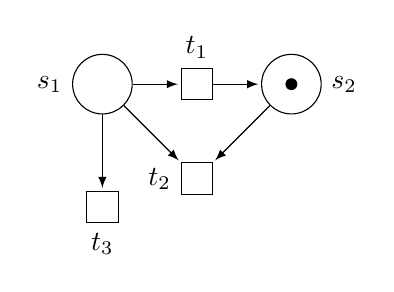
\begin{tikzpicture}[x=1.2cm,y=-1.2cm,baseline=(t1),>=latex]
    \node[place,label=left:$s_1$]  (s1) at (-1.0,0) {} ;
    \node[place,tokens=1,label=right:$s_2$] (s2) at ( 1.0,0) {} ;
    \node[transition,label=above:$t_1$] (t1) at (0,0) {}
    edge[pre]  (s1)
    edge[post] (s2) ;
    \node[transition,label=left:$t_2$] (t2) at (0,1) {}
    edge[pre] (s1)
    edge[pre] (s2);
    \node[transition,label=below:$t_3$] (t3) at (-1,1.3) {}
    edge[pre] (s1) ;
  \end{tikzpicture}
\end{center}
and Alloy is asked to complete/extend it while satisfying a set of constraints such as (combinations of some of the following):
\begin{itemize}
\item
  maximum number of places to add
\item
  maximum number of transitions to add
\item
  maximum number of tokens to add, per place or overall
\item
  maximum change in weights that is allowed
\item
  presence or absence of self-loops
\item
  presence or absence of sink and/or source transitions
\item
  number of activated transitions
\item
  presence or absence of conflicts
\item
  presence or absence of concurrently activated transitions
\item
  \dots
\end{itemize}

\end{document}

% ---------------------------------------------------------------------------- %
%% Local Variables:
%% coding: utf-8
%% ispell-local-dictionary: "british"
%% End:
